\documentclass{article}

%%% Fill details here (in the second brackets)
\newcommand{\name}{Sam Teeter}     % Your name (First Last)
\newcommand{\wustlkey}{teeters}             % Your WUSTL Key
%%%



%%%%%%%%%%%%%%%%%%%%%% Formatting Stuff %%%%%%%%%%%%%%%%%%%%%%%%%%%
\usepackage{times}
\usepackage[T1]{fontenc}

\setlength{\parskip}{1em}\setlength{\parindent}{0pt}
\linespread{1.25}
\usepackage[margin=0.7in,top=1in]{geometry}\usepackage{fancyhdr}
\pagestyle{fancy}\lhead{\bf \name}\rhead{\bf \wustlkey}\cfoot{\thepage}
\newcommand{\info}{\clearpage \subsection*{Information}}
\newcommand{\solution}[1]{\clearpage \subsection*{Solution #1}}
\newcommand{\spart}[1]{\paragraph{(#1)}}
%%%%%%%%%%%%%%%%%%%%%%%%%%%%%%%%%%%%%%%%%%%%%%%%%%%%%%%%%%%%%%%%%%%


%%% Add any more packages if you want to
\usepackage{amsmath,graphicx}


\begin{document}
%%%%% Main Body goes here

% Begin solution to every problem like this.
\solution{1}

\spart{a} Where 
\begin{equation} 
I = gI^0 + g\sqrt{I^0} \epsilon_1 + \sqrt{g^2 \sigma_{2a}^2+\sigma_{2b}^2} \epsilon_2
\end{equation}
we can write the total noise $\epsilon$ as
\begin{equation}
\epsilon = g\sqrt{I^0} \epsilon_1 + \sqrt{g^2 \sigma_{2a}^2+\sigma_{2b}^2} \epsilon_2
\end{equation}
Since this is a linear combination of the random variables $\epsilon_1, \epsilon_2 ~ N(0,1)$ we have
\begin{align}
\mu_{\epsilon} &= 0 \\
\sigma^2_\epsilon &= g^2I^0 + g^2\sigma^2_{2a} + \sigma^2_{2b}
\end{align}


\spart{b} Given exposure time $T/k$, if the amplification $g^{(k)} = gk$, the new variance of the noise will be
\begin{equation}
\sigma^2_{\epsilon(k)} = g^2k^2I^0 + g^2k^2\sigma^2_{2a} + \sigma^2_{2b}
\end{equation}

\spart{c} We can express our final, average image as 
\begin{align}
I &= \frac{1}{k} \sum_k( gI^0_k + \epsilon_k) \\
  &= gI^0 + \frac{1}{k} \sum_k \epsilon_k
\end{align}
Therefore
\begin{equation}
\epsilon = \frac{1}{k} \sum_k \epsilon_k
\end{equation}
We already know the variance of each $\epsilon_k$ from equation (4). Since $\epsilon$ is a sum of independent random variables, we can therefore write
\begin{align}
\sigma^2_\epsilon &= \sum_k \frac{1}{k^2} \sigma^2_{\epsilon_k} \\
 &= \sum_k \frac{1}{k^2} \left( g^2I^0 + g^2\sigma^2_{2a} + \sigma^2_{2b} \right)\\
 &= \frac{1}{k} \left( g^2I^0 + g^2\sigma^2_{2a} + \sigma^2_{2b} \right)
\end{align}

\spart{d} If we look back to equation (1), we notice that while the ideal image $gI^0$ scales with $I^0$, the error $e$ scales with $\sqrt{I^0}$, meaning that since $I^0$ scales linearly with $T$, the signal-to-noise ratio will always be higher with a longer exposure time. However, as the equation above shows, the variance of the noise decreases as the number of shots increases, meaning that on average the noise will be closer to its mean value of 0. Which is preferable depends on the photographer's goal: high ISO gain or low average noise. 

\solution{2} Here is my input image and output after histogram equalization.

\begin{figure*}[!h]
  \centering
  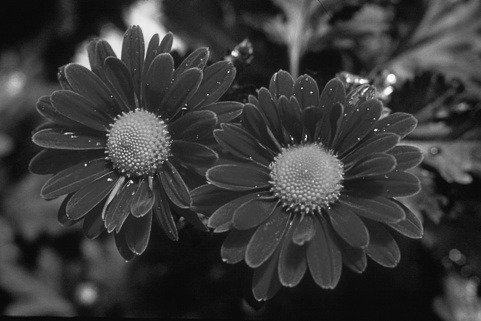
\includegraphics[height=10em]{code/inputs/p2_inp.png}
  \caption{Input image}
\end{figure*}

\begin{figure*}[!h]
  \centering
  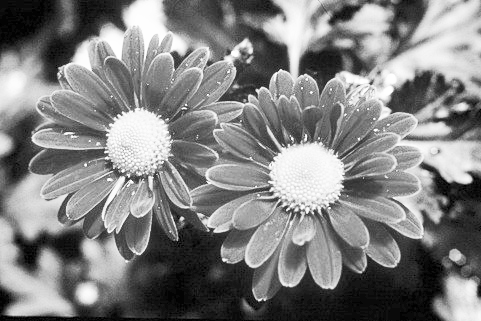
\includegraphics[height=10em]{code/outputs/prob2.png}
  \caption{Equalized image}
\end{figure*}

\solution{3}

\spart{a} Input and output for gradient mapping using the Sobel kernel:

\begin{figure*}[!h]
  \centering
  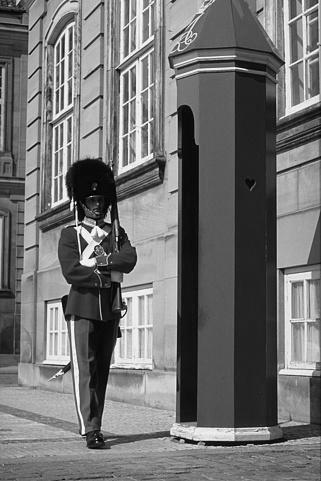
\includegraphics[height=10em]{code/inputs/p3_inp.png}
  \caption{Input image}
\end{figure*}

\begin{figure*}[!h]
  \centering
  
\includegraphics[height=10em]{code/outputs/prob3_a.png}
  \caption{Gradient map}
\end{figure*}

\spart{b} Edge images before NMS:

\begin{figure*}[!h]
  \centering
  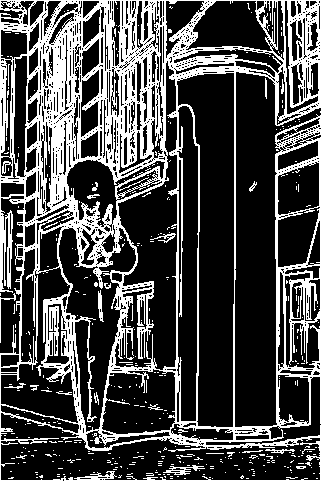
\includegraphics[height=10em]{code/outputs/prob3_b_0.png}
  \caption{Low threshold}
\end{figure*}

\begin{figure*}[!h]
  \centering
  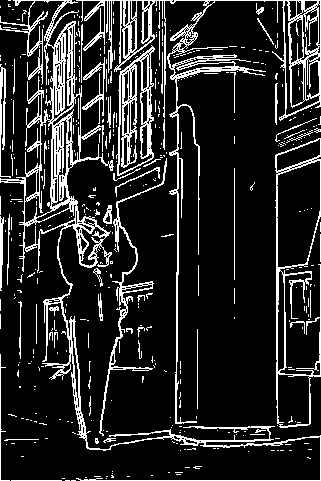
\includegraphics[height=10em]{code/outputs/prob3_b_1.png}
  \caption{Medium threshold}
\end{figure*}

\begin{figure*}[!h]
  \centering
  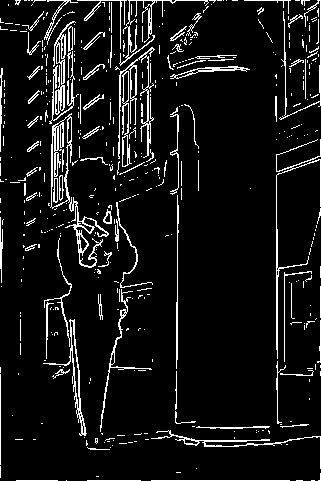
\includegraphics[height=10em]{code/outputs/prob3_b_2.png}
  \caption{High threshold}
\end{figure*}

Edge images after NMS:

\begin{figure*}[!h]
  \centering
  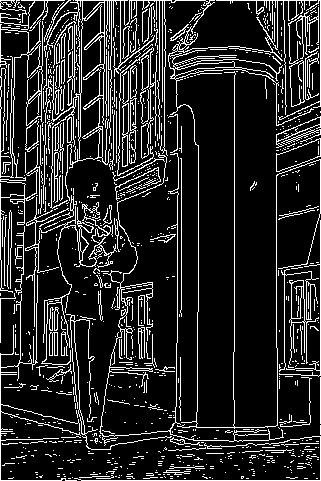
\includegraphics[height=10em]{code/outputs/prob3_b_nms0.png}
  \caption{Low threshold}
\end{figure*}

\begin{figure*}[!h]
  \centering
  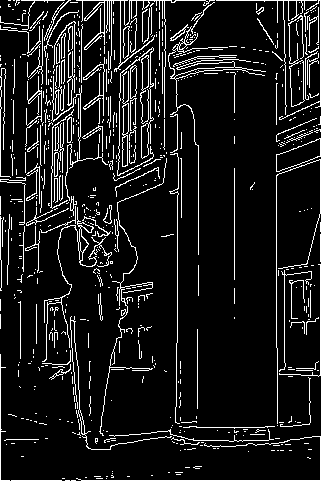
\includegraphics[height=10em]{code/outputs/prob3_b_nms1.png}
  \caption{Medium threshold}
\end{figure*}

\begin{figure*}[!h]
  \centering
  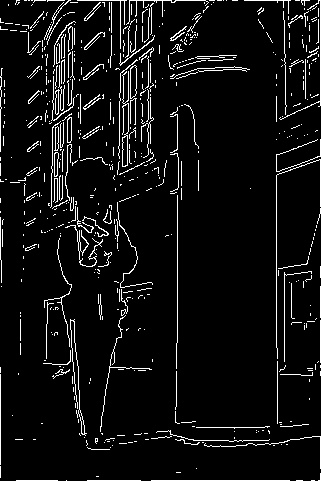
\includegraphics[height=10em]{code/outputs/prob3_b_nms2.png}
  \caption{High threshold}
\end{figure*}

\solution{4}

Inputs and outputs for bilateral filtering:

\begin{figure*}[!h]
  \centering
  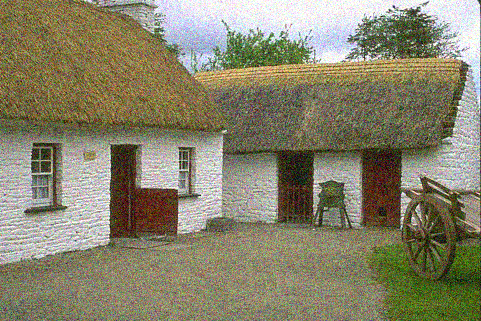
\includegraphics[height=10em]{code/inputs/p4_nz1.png}
  \caption{Input 1}
\end{figure*}

\begin{figure*}[!h]
  \centering
  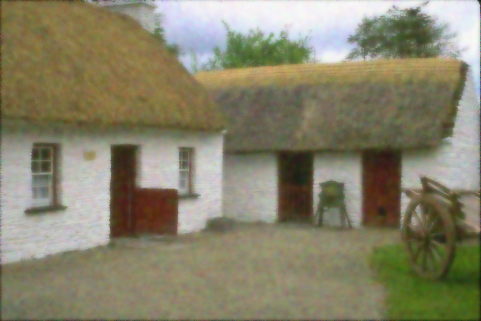
\includegraphics[height=10em]{code/outputs/prob4_1_a.png}
  \caption{Output 1a}
\end{figure*}

\begin{figure*}[!h]
  \centering
  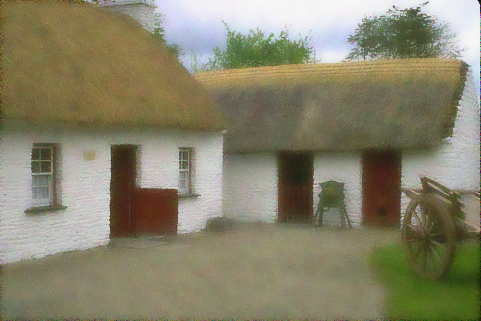
\includegraphics[height=10em]{code/outputs/prob4_1_b.png}
  \caption{Output 1b}
\end{figure*}

\begin{figure*}[!h]
  \centering
  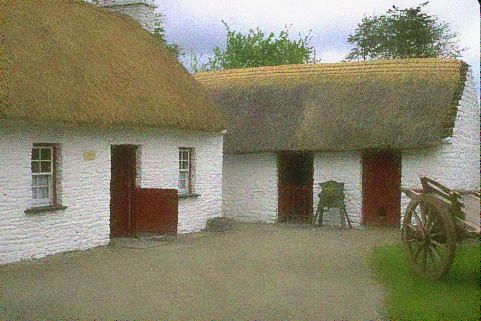
\includegraphics[height=10em]{code/outputs/prob4_1_c.png}
  \caption{Output 1c}
\end{figure*}

\begin{figure*}[!h]
  \centering
  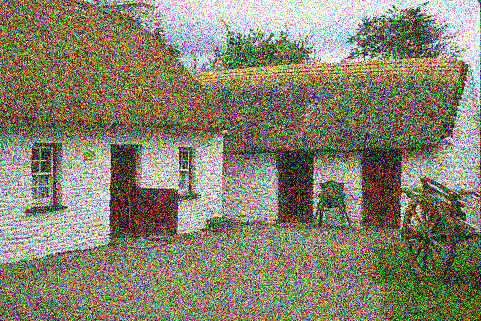
\includegraphics[height=10em]{code/inputs/p4_nz2.png}
  \caption{Input 2}
\end{figure*}

\begin{figure*}[!h]
  \centering
  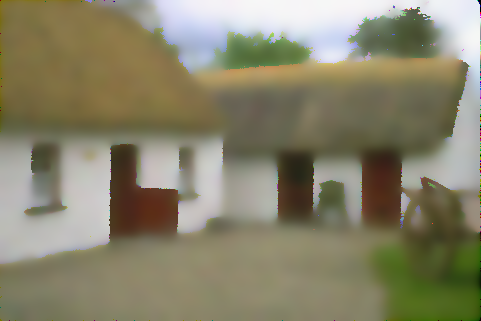
\includegraphics[height=10em]{code/outputs/prob4_1_rep.png}
  \caption{Image 1: repeated filtering}
\end{figure*}

\begin{figure*}[!h]
  \centering
  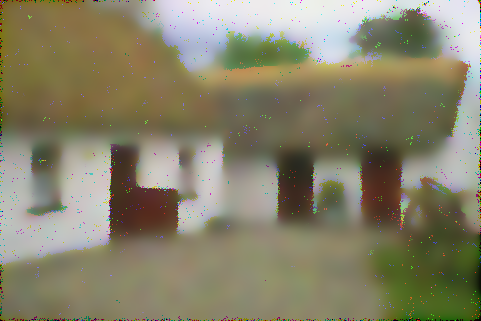
\includegraphics[height=10em]{code/outputs/prob4_2_rep.png}
  \caption{Image 2: repeated filtering}
\end{figure*}



\solution{5}

\spart{a} Consider the discrete Fourier transform $F[u,v]$:
\begin{equation}
F[u,v] = \frac{1}{WH} \sum_{x,y} X[x,y] \text{exp} \left(-i2\pi \left( \frac{ux}{w} + \frac{vy}{H} \right) \right) 
\end{equation}
Substituting $q$ for $2\pi\left( \frac{ux}{W} + \frac{vy}{H} \right)$ and applying Euler's formula this becomes
\begin{equation}
F[u,v] = \frac{1}{WH} \sum_{x,y} X[x,y]\left( \cos q + i\sin q \right)
\end{equation}
We can therefore think of each value of $F$ as two scalars, the real sum of cosines and the imaginary sum of sines.

 From the symmetry of the Fourier transform, we know that
\begin{equation}
F[W-u, H-v] = F[-u, -v] = \frac{1}{WH} \sum_{x,y} X[x,y]\left( \cos(-q) + i\sin(-q) \right)
\end{equation}
Applying the odd and even properties of sine and cosine, we get
\begin{equation}
F[W-u, H-v] = F[-u, -v] = \frac{1}{WH} \sum_{x,y} X[x,y]\left( \cos(q) - i\sin(q) \right)
\end{equation}

This means that half the values in $F$, represented by their real and imaginary components $r_{u,v} + i_{u,v}$, can be used to calculate the other half, $r_{W-u, H-v} - i_{W-u, H-v}$. Consider these examples:

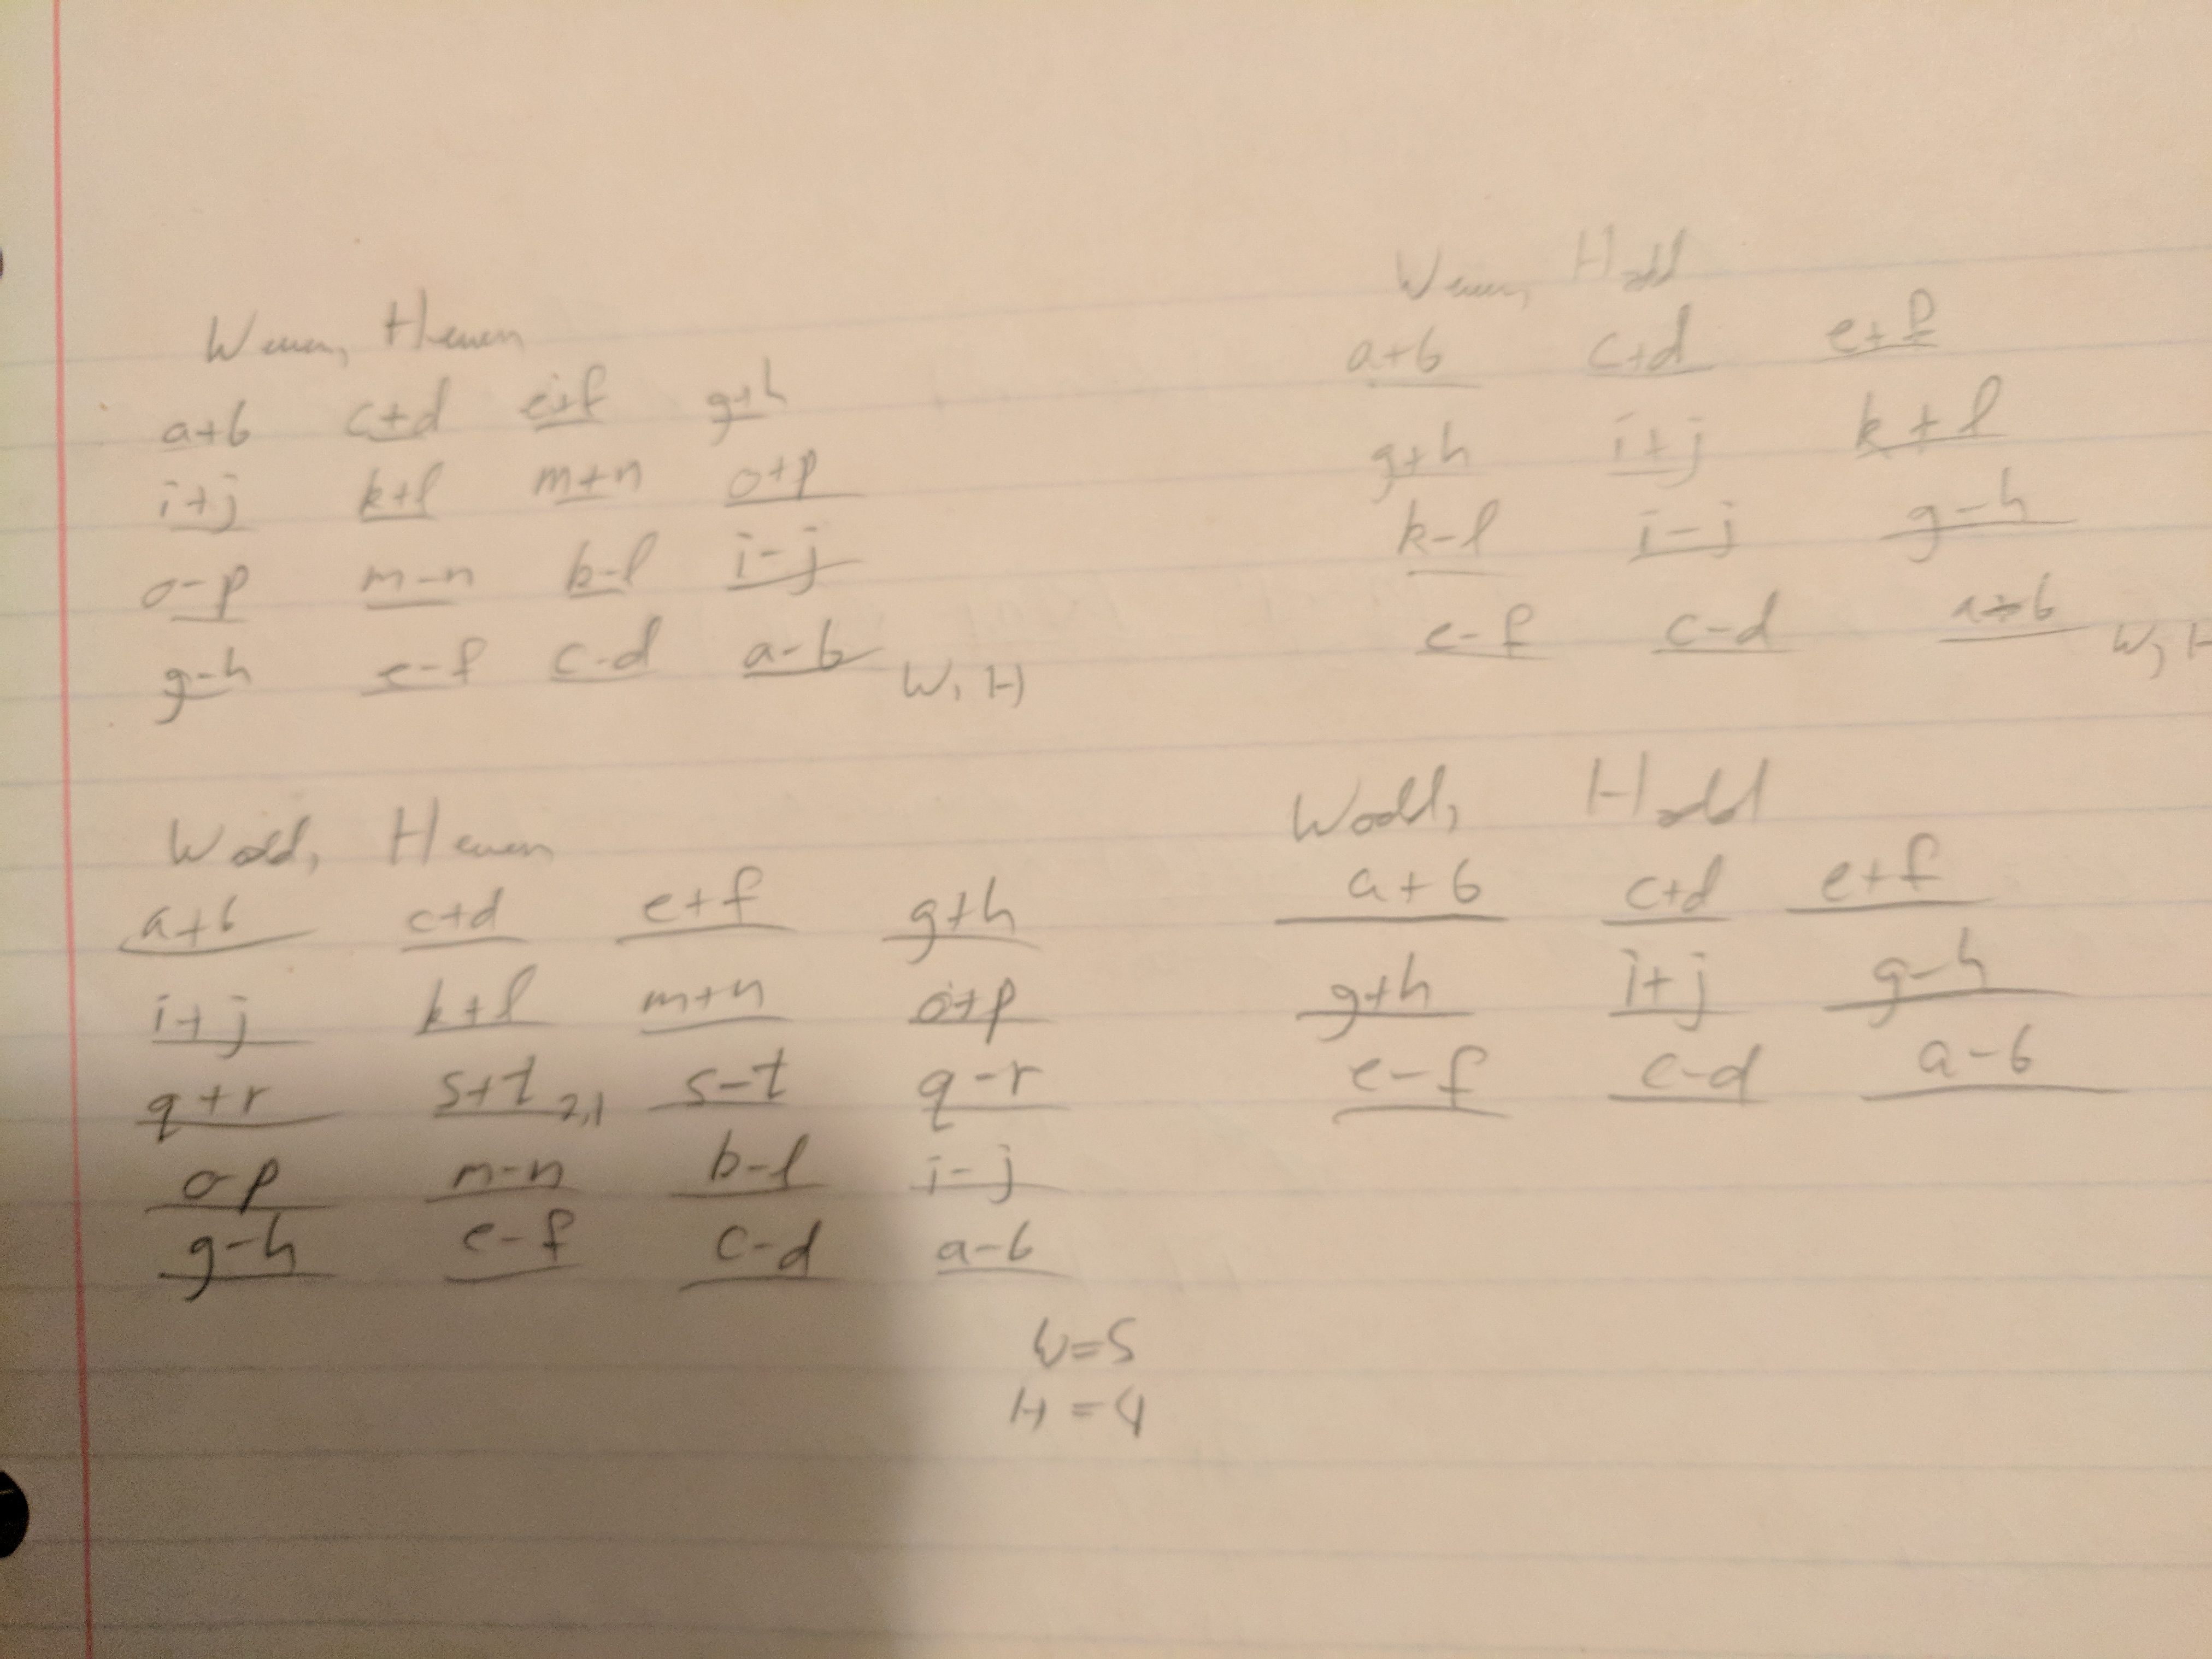
\includegraphics[width=\textwidth]{prob5_examples.jpg}

If we read each matrix from left to right and top to bottom, we see that the matched pairs of terms form a reflected sequence. We can therefore store the imaginary and real components for the first $W*H$ terms, and we can retrieve the other terms by flattening our stored terms into a sequence $(r_1 + i_1) ... (r_{WH/2}+i_{WH/2})$, computing the second sequence $(r_1 - i_1) ... (r_{WH/2}-i_{WH/2})$, inverting that sequence, attaching it to the end of the first sequence, and shaping the resulting long list into a matrix. The only exception to this rule is when the total number of elements in the transform matrix is odd, which occurs if and only if both $W$ and $H$ are odd. In this case, we will need to store the scalars up to the central element $(r+i)_{\text{ceiling}(WH/2)}$, but only reflect the elements before it in the sequence, $(r+i)_{1}...(r+i)_{\text{floor}(WH/2)}$. 

\spart{b} Output from prob5.py:

\begin{figure*}[!h]
  \centering
  
\includegraphics[height=10em]{code/outputs/prob5.png}
  \caption{Convolution in the Fourier domain}
\end{figure*}

\solution{6}

\spart{a} Haar wavelet pyramid:

\begin{figure*}[!h]
  \centering
  
\includegraphics[height=10em]{code/outputs/prob6a_1.png}
  \caption{N=1}
\end{figure*}

\begin{figure*}[!h]
  \centering
  
\includegraphics[height=10em]{code/outputs/prob6a_2.png}
  \caption{N=2}
\end{figure*}


\begin{figure*}[!h]
  \centering
  
\includegraphics[height=10em]{code/outputs/prob6a_3.png}
  \caption{N=3}
\end{figure*}
\info

\spart{b} Reconstructing the original image:

\begin{figure*}[!h]
  \centering
  
\includegraphics[height=10em]{code/outputs/prob6b_2.png}
  \caption{L3}
\end{figure*}

\begin{figure*}[!h]
  \centering
  
\includegraphics[height=10em]{code/outputs/prob6b_1.png}
  \caption{L2}
\end{figure*}

\begin{figure*}[!h]
  \centering
  
\includegraphics[height=10em]{code/outputs/prob6b_0.png}
  \caption{L1}
\end{figure*}

\begin{figure*}[!h]
  \centering
  
\includegraphics[height=10em]{code/outputs/prob6b.png}
  \caption{L0 (original image)}
\end{figure*}

This problem set took approximately 16 hours of effort.


I discussed this problem set with:
\begin{itemize}
\item Jarett Gross
\end{itemize}


% Note that you might have to escape some special symbols in URLS like \_
I also got hints from the following sources:
\begin{itemize}
\item Numpy documentation at https://docs.scipy.org/
\item Old paper on Haar wavelets at https://www.eecis.udel.edu/~amer/CISC651/Haar.wavelets.paper.by.Mulcahy.pdf

\end{itemize}

\end{document}
